\chap{Circuit Design with Altium Designer}
\section{Introduction}
Altium Designer is an electronic design
automation software package for printed circuit board (PCB), FPGA and embedded software design, and associated library and release management automation. A Printed Circuit Board (PCB) mechanically supports and electrically connects electric components using conductive tracks, pads and other features etched from copper sheets laminated onto a non-conductive substrate.

\begin{figure}[!htp]
    \centering
    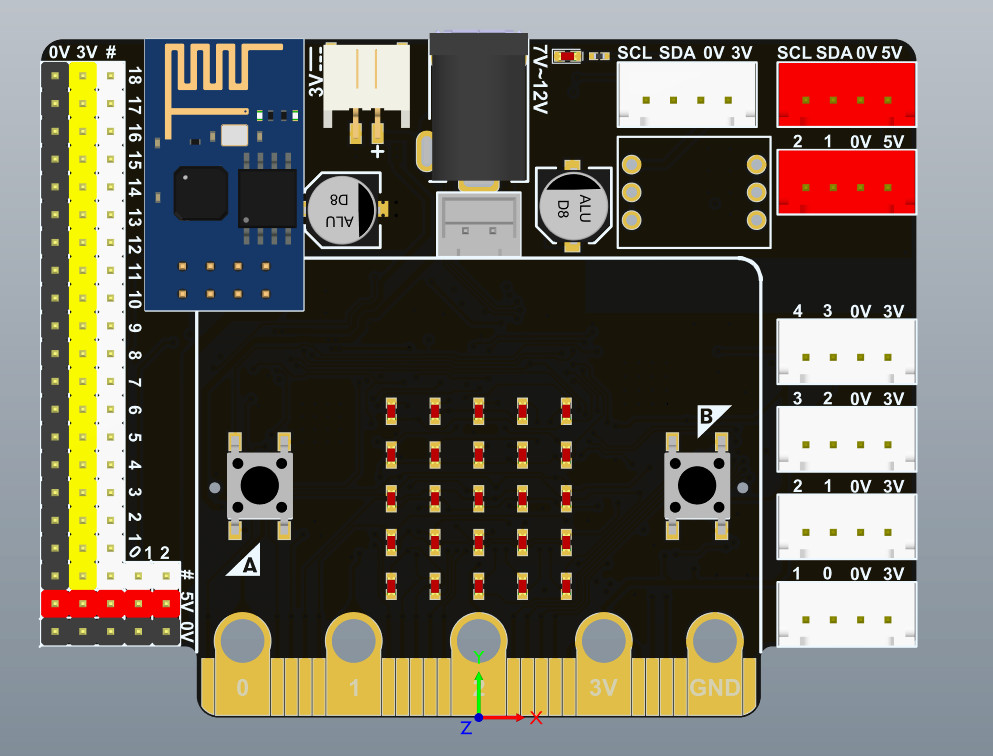
\includegraphics[width=4in]{source/picture/bai_4/bbc_altium.jpg}
    \caption{\textit{PCB circuit in Altium Designer}}
    \label{bai4_pic}
\end{figure}


In this lab, two different voltage regular circuits are designed in Altium, based on IC 7805 and LM2596. \textbf{The manuals are provided by videos}.

\section{Voltage Regulator using 7805}
Voltage regulator like IC7805 belongs to the 78xx series ICs. In the 78xx series, xx represents the fixed output voltage value and 7805 is a fixed linear voltage regulator. Batteries provide a voltage of 1.2V, 3.7V, 9V, and 12V. This voltage is good for the circuits which voltage requirements are in that range. The regulated power supply in this regulator is +5V DC. \\

\begin{figure}[!htp]
    \centering
    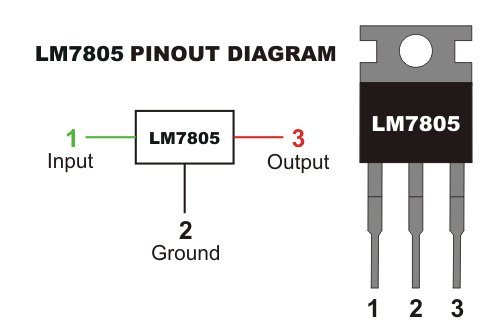
\includegraphics[width=3in]{source/picture/bai_4/LM7805_PinOut.jpg}
    \caption{\textit{LM7805 Pin Out}}
    \label{bai4_pic1}
\end{figure}

The 7805 voltage regulator is a three-terminal voltage regulator IC. In various applications, a 7805 voltage regulator with a fixed output voltage is used. The availability of this is through various packages like SOT-223, TO-263, TO-220, and TO-3. Among this, TO-220 is the most used one. The pin diagram of 7805 voltage regulator IC and its description are explained bellow:
\begin{itemize}
    \item \textbf{Pin1 - Input}: This is an input pin and the voltage range should be between 7V to 35V. an unregulated voltage is applied to this input pin for regulation. The pin will receive its maximum efficiency at 7.2V input.
    \item \textbf{Pin 2 - Ground}: Pin2 is the ground pin, it means the ground is connected to this pin. Input and output are common to it.
    \item \textbf{Pin 3 - Output}: Pin3 is the output pin, where the regulated output is taken by this pin. It is about 5V(4.8V to 5.2V)
\end{itemize}

\begin{figure}[!htp]
    \centering
    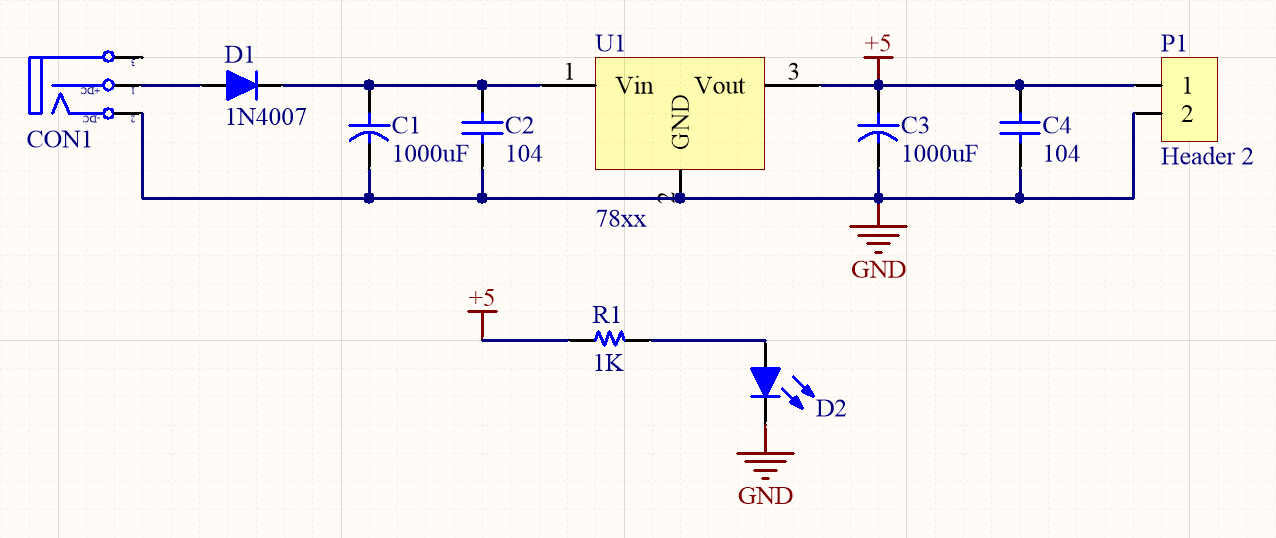
\includegraphics[width=5in]{source/picture/bai_4/7805_SCH.PNG}
    \caption{\textit{Voltage regulator using 78xx schematic in Altium Designer}}
    \label{bai4_pic2}
\end{figure}

The basic circuit of 7805 is very simple. It just needs two capacitors if the input is unregulated DC voltage, even the two capacitors used are also not mandatory. This 7805 circuit is capable of upholding fixed output voltage even if some changes take place in input voltage.\\

The manual for this circuit is posted at the link bellow:
\begin{center}
    \link{https://www.youtube.com/watch?v=mSEBrma5MNM}
\end{center}

\subsection{Schematic design}
Students are proposed to capture the schematic design in Altium Designer and place the image in this part.\\

Some hot keys are normally used in the schematic is the space bar, X( horizontal mirror), Y (vertial mirror) and Ctrl + W (place a wire).\\

\textbf{\textit{Your image goes here}}

\subsection{PCB layout}
Similarly to the schematic, some snap shorts of for the TOP, BOTTOM layers are required in this report. Moreover, several 3D images of your schematic are also required.\\

A manual video can be found at:
\begin{center}
    \link{https://www.youtube.com/watch?v=PW\_QQpoODDk}
\end{center}

\textbf{\textit{Your image goes here}}


\section{Volatage Regulator using LM2596}

LM2596 is a voltage regulator mainly used to step down the voltage or to drive load under 3A. It is also known as DC-to-DC power converter or buck converter which is used to step down the voltage from its input supply to the output load. The current goes up during this voltage step down process.\\


LM2596 comes with a remarkable load and line regulation. It is available in both versions: fixed output voltage version with 3.3V, 5V, 12V, and customized output version where you can choose the output as per your requirement. This regulator is incorporated with a fixed-frequency oscillator and an internal frequency compensation method.\\

The typical connection for LM2596 is proposed by Texas Instrument (TI), as following:

\begin{figure}[!htp]
    \centering
    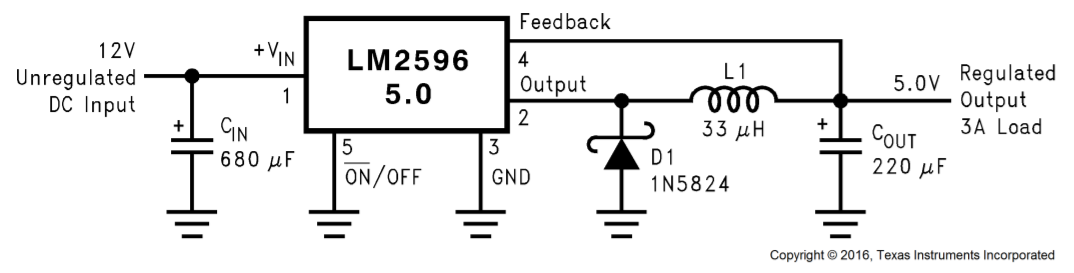
\includegraphics[width=5in]{source/picture/bai_4/LM2596.PNG}
    \caption{\textit{Typical connection for LM2596}}
    \label{bai4_pic3}
\end{figure}

This circuit is simulated in PSpice in previous lab, and is implemented in Altium Design in this lab. The introduction of this circuit is presented in the video bellow:
\begin{center}
    \link{https://www.youtube.com/watch?v=57Ra92p3C0k}
\end{center}
\subsection{Schematic design}
Students are proposed to capture the schematic design in Altium Designer and place the image in this part.\\

Some hot keys are normally used in the schematic is the space bar, X( horizontal mirror), Y (vertial mirror) and Ctrl + W (place a wire).\\

The manual is posted in this link:

\begin{center}
    \link{https://www.youtube.com/watch?v=DGiHsGWPyYw}
\end{center}


\textbf{\textit{Your image goes here}}

\subsection{PCB layout}
Similarly to the schematic, some snap shorts of for the TOP, BOTTOM layers are required in this report. Moreover, several 3D images of your schematic are also required.\\

The manual is posted in this link:\\

\begin{center}
    \link{https://www.youtube.com/watch?v=WXszMiTSGPo}
\end{center}

\textbf{\textit{Your image goes here}}